

%
% -----
% The full Finite State Automata over inference states
% -----
%
\newcommand\completeFSA{
  \begin{tikzpicture}[shorten >=1pt,node distance=2.0cm,auto,semithick,inner sep=2pt,bend angle=15,
    % (styles)
    every state/.style={draw=red!100,very thick,fill=red!10},
    accepting/.style={draw=blue!50,very thick,fill=blue!10},
    initial/.style={draw=green!90,very thick,fill=green!10}
    ]

    % (states)
    \node[state,initial]   (equivalent)                             {\equivalent};
    \node[state,accepting] (reverse)    [above right=of equivalent] {\reverse};
    \node[state,accepting] (cover)      [right=of reverse]          {\cover};
    \node[state]           (negate)     [below right=of cover]      {\negate};
    \node[state,initial]   (forward)    [below right=of equivalent] {\forward};
    \node[state]           (alternate)  [right=of forward]          {\alternate};

    % (paths)
    \path[->]  (equivalent) edge              node {\negate}             (negate);
    \path[->]  (negate)     edge [bend right] node {\forward}            (cover)
                            edge [bend left]  node {\alternate}          (reverse)
                            edge [bend left]  node {\reverse}            (alternate)
                            edge [bend right] node {\cover}              (forward)
                            edge [loop right] node {\equivalent}         (negate)
               (reverse)    edge [bend left]  node {\negate\cover}       (cover)
                            edge [loop above] node {\reverse\equivalent} (reverse)
               (cover)      edge [bend left]  node {\negate\alternate}   (reverse)
                            edge [loop above] node {\forward\equivalent} (cover)
               (forward)    edge [bend left] node {\negate\alternate}   (alternate)
                            edge [loop below] node {\forward\equivalent} (forward)
               (alternate)  edge [bend left]  node {\negate\cover}       (forward)
                            edge [loop below] node {\reverse\equivalent} (alternate)
               ;
  \end{tikzpicture}
}

%
% -----
% A Finite State Automata for the collapsed inference states
% -----
%
\newcommand\collapsedFSAImpl[3]{
  \begin{tikzpicture}[shorten >=1pt,node distance=2.0cm,auto,semithick,inner sep=2pt,bend angle=30,
    % (styles)
    every state/.style={draw=red!100,very thick,fill=red!#1},
    accepting/.style={draw=blue!50,very thick,fill=blue!#3},
    initial/.style={draw=green!90,very thick,fill=green!#2}
    ]

    % (states)
    \node[state,initial]   (valid)                               {$~~\varphi \Rightarrow \psi~~$};
    \node[state,accepting] (unknown)    [above right=of valid]   {$~~\varphi \nRightarrow \psi~~$};
    \node[state]           (invalid)    [below right=of unknown] {$\varphi \Rightarrow \lnot \psi$};
    
    % (edges)
    \path[->]  (valid)      edge [bend left]  node {\negate\alternate}   (invalid)
                            edge [bend left]  node {\reverse\cover}      (unknown)
                            edge [loop left]  node {\equivalent\forward} (valid)
               (invalid)    edge [bend left]  node {\negate\cover}       (valid)
                            edge [bend right] node {\alternate\forward}  (unknown)
                            edge [loop right] node {\equivalent\reverse} (invalid)
               (unknown)    edge [loop above] node {any}                 (unknown)
               ;

  \end{tikzpicture}
}

\newcommand\collapsedFSA{\collapsedFSAImpl{10}{10}{10}}
\newcommand\collapsedFSARed{\collapsedFSAImpl{50}{10}{10}}
\newcommand\collapsedFSAGreen{\collapsedFSAImpl{10}{50}{10}}
\newcommand\collapsedFSABlue{\collapsedFSAImpl{10}{10}{50}}

%
% -----
% A Teaser Search Path
% -----
%
\newcommand\teaserSearch{
  \tikzstyle{level 1}=[level distance=2.0cm, sibling distance=3.5cm]
  \tikzstyle{level 2}=[level distance=2.0cm, sibling distance=2cm]
  \tikzstyle{level 3}=[level distance=2.0cm, sibling distance=2cm]
  \tikzstyle{level 4}=[level distance=2.0cm, sibling distance=2cm]
  \tikzstyle{fact} = [text width=7em, text centered]
  \tikzstyle{sink} = [text width=7em, text centered, 
                      rectangle, draw]
  \tikzset{
    goodPath/.style={draw=blue}
  }

  % "No carnivores eat animals"
  % false because: "The cat ate a mouse"

  \begin{tikzpicture}[grow=down, sloped]
  \node[fact] {\w{No carnivores eat animals?}}
    child {
      node[fact] {\w{\textbf{The} carnivores eat animals}} 
      child {
        node[fact] {\w{The \textbf{cat} \\ eats animals}} 
        child {
          node[fact] {\w{The cat \\ ate \textbf{an} animal}}
          child {
            node[sink] {\w{The cat \\ ate a \textbf{mouse}}} 
            edge from parent [goodPath] node[below] {\rotatebox{90}{$\reverse$}}
          }
          edge from parent [goodPath] node[below] {\rotatebox{90}{$\equivalent$}}
        }
        edge from parent [goodPath] node[below] {$\rotatebox{90}{\reverse}$}
      }
      edge from parent [goodPath] node[above] {$\rotatebox{340}{\negate}$}
    }
    child {
      node[fact] {\w{No \textbf{animals} \\ eat animals}} 
      child {
        node[fact] {\w{No animals \\ eat \textbf{things}}}
          [clockwise from=-50,sibling angle=20]
          child foreach \x in {1,2,3,4} {
            [clockwise from=-55,sibling angle=20]
%            child foreach \x in {1,2,3,4} {}
          }
        edge from parent node[above,shift={(-1 ex,0 ex)}] {$\rotatebox{-63}{\reverse}$}
      }
      child {
        node[fact] {$\dots$}
      }
      edge from parent node[below] {$\rotatebox{90}{\reverse}$}
    }
    child {
      node[fact] {$\dots$}
    };
  \end{tikzpicture}
}

%
% -----
% Teaser Search Paths For Presentation
% -----
%
\def\setstyles{
  \tikzstyle{level 1}=[level distance=1.5cm, sibling distance=3.5cm]
  \tikzstyle{level 2}=[level distance=1.5cm, sibling distance=2cm]
  \tikzstyle{level 3}=[level distance=1.5cm, sibling distance=2cm]
  \tikzstyle{level 4}=[level distance=1.5cm, sibling distance=2cm]
  \tikzstyle{fact} = [text width=7em, text centered, line width=2pt]
  \tikzstyle{boxfact} = [text width=7em, text centered, line width=2pt,
                         rectangle, draw=black, line width=1pt]
  \tikzstyle{shortfact} = [text width=3em, text centered, line width=2pt]
  \tikzstyle{sink} = [text width=7em, text centered, 
                      rectangle, draw=blue, line width=2pt]
  \tikzstyle{unksink} = [text width=7em, text centered, 
                      rectangle, draw=blue]
  \tikzstyle{othersink} = [text width=5em, text centered, 
                      rectangle, draw=blue]
  \tikzset{
    goodPath/.style={draw=blue}
  }
  \tikzset{
    goodPathDown/.style={draw=blue,->}
  }
  \tikzset{
    goodPathUp/.style={draw=blue,<-}
  }
  \tikzset{
    strongPath/.style={draw=blue, line width=3pt}
  }
}

\def\setstylesposter{
  \tikzstyle{level 1}=[level distance=3.75cm, sibling distance=8.5cm]
  \tikzstyle{level 2}=[level distance=3.75cm, sibling distance=4.75cm]
  \tikzstyle{level 3}=[level distance=3.75cm, sibling distance=4.75cm]
  \tikzstyle{level 4}=[level distance=3.75cm, sibling distance=4.75cm]
  \tikzstyle{fact} = [text width=7em, text centered, line width=2pt]
  \tikzstyle{boxfact} = [text width=7em, text centered, line width=2pt,
                         rectangle, draw=black, line width=1pt]
  \tikzstyle{shortfact} = [text width=3em, text centered, line width=2pt]
  \tikzstyle{sink} = [text width=7em, text centered, 
                      rectangle, draw=blue, line width=2pt]
  \tikzstyle{unksink} = [text width=7em, text centered, 
                      rectangle, draw=blue]
  \tikzstyle{othersink} = [text width=5em, text centered, 
                      rectangle, draw=blue]
  \tikzset{
    goodPath/.style={draw=blue}
  }
  \tikzset{
    goodPathDown/.style={draw=blue,->}
  }
  \tikzset{
    goodPathUp/.style={draw=blue,<-}
  }
  \tikzset{
    strongPath/.style={draw=blue, line width=3pt}
  }
}

\def\teaserPremises{
  \node[right = of main](db){
\includegraphics[height=2.2cm]{../img/database.png}};
  \node[othersink, right = of main](tails) {\w{All cats have tails}};
  \node[othersink, right = of tails](kittens) {\w{All kittens are cute}};
  \draw (db.north west) -- (main.north west);
  \draw (db.south west) -- (main.south west);
  \draw (db.north east) -- (kittens.north east);
  \draw (db.south east) -- (kittens.south east);
}

\def\teaserPremisesPoster{
  \node[right = of main](db){
\includegraphics[height=4.5cm]{../img/database.png}};
  \node[othersink, right = of main](tails) {\w{All cats have tails}};
  \node[othersink, right = of tails](kittens) {\w{All kittens are cute}};
  \draw (db.north west) -- (main.north west);
  \draw (db.south west) -- (main.south west);
  \draw (db.north east) -- (kittens.north east);
  \draw (db.south east) -- (kittens.south east);
}

\newcommand\teaserManyPremises{
  \setstyles

  \begin{tikzpicture}[grow=down, sloped]
  \node[unksink](main) {\w{The cat ate a mouse}};
  \teaserPremises
  \end{tikzpicture}
}

\newcommand\teaserBlindInferenceNaturalOrderBlind{
  \setstyles

  \begin{tikzpicture}[grow=down, sloped]
  \node[sink](main) {\w{The cat ate a mouse}}
    child {
      node[fact] {$\dots$} 
      child {
        node[fact] {$\dots$} 
        child {
          node[fact] {
\includegraphics[height=0.75cm]{../img/fact.jpg}}
          edge from parent [goodPathDown] node[below] {\rotatebox{90}{}}
        }
        edge from parent [goodPathDown] node[below] {\rotatebox{90}{}}
      }
      edge from parent [goodPathDown] node[below] {\rotatebox{90}{}}
    };
  \teaserPremises
  \end{tikzpicture}
}

\newcommand\teaserBlindInferenceNaturalOrder{
  \setstyles

  \begin{tikzpicture}[grow=down, sloped]
  \node[sink](main) {\w{The cat ate a mouse}}
    child {
      node[fact] {$\dots$} 
      child {
        node[fact] {$\dots$} 
        child {
          node[fact] {\false{No carnivores eat animals}} 
          edge from parent [goodPathDown] node[below] {\rotatebox{90}{}}
        }
        edge from parent [goodPathDown] node[below] {\rotatebox{90}{}}
      }
      edge from parent [goodPathDown] node[below] {\rotatebox{90}{}}
    };
  \teaserPremises
  \end{tikzpicture}
}

\def\glass{
\includegraphics[height=0.75cm]{../img/magnifying_glass.png}}
\def\glassposter{
\includegraphics[height=2.0cm]{../img/magnifying_glass.png}}

\newcommand\teaserBlindInference{
  \setstyles

  \begin{tikzpicture}[grow=down, sloped]
  \node[fact](query) {\w{No carnivores eat animals?}}
    child {
      node[fact] {$\dots$} 
      child {
        node[fact] {$\dots$}
        child {
          node[sink](main) {\w{The cat \\ ate a \textbf{mouse}}} 
          edge from parent [goodPathUp] node[below] {}
        }
        edge from parent [goodPathUp] node[below] {}
      }
      edge from parent [goodPathUp] node[below] {}
    };
  \teaserPremises
  \node[right = of query]{\hspace{-1.75cm}\glass};
  \end{tikzpicture}
}

\newcommand\teaserInference{
  \setstyles

  \begin{tikzpicture}[grow=down, sloped]
  \node[fact](query) {\w{No carnivores eat animals?}}
    child {
      node[fact] {\w{\textbf{The} carnivores eat animals}} 
      child {
        node[fact] {\w{The \textbf{cat} \\ eats animals}} 
        child {
          node[fact] {\w{The cat \\ ate \textbf{an} animal}}
          child {
            node[sink](main) {\w{The cat \\ ate a \textbf{mouse}}} 
            edge from parent [goodPath] node[below] {\rotatebox{90}{}}
          }
          edge from parent [goodPath] node[below] {\rotatebox{90}{}}
        }
        edge from parent [goodPath] node[below] {\rotatebox{90}{}}
      }
      edge from parent [goodPath] node[below] {\rotatebox{90}{}}
    };
  \teaserPremises
  \node[right = of query]{\hspace{-1.75cm}\glass};
  \end{tikzpicture}
}

\newcommand\teaserFullDerivation{
  \setstyles

  \begin{tikzpicture}[grow=down, sloped]
  \node[fact](query) {\w{No carnivores eat animals?}}
    child {
      node[fact] {\w{\textbf{The} carnivores eat animals}} 
      child {
        node[fact] {\w{The \textbf{cat} \\ eats animals}} 
        child {
          node[fact] {\w{The cat \\ ate \textbf{an} animal}}
          child {
            node[sink](main) {\w{The cat \\ ate a \textbf{mouse}}} 
            edge from parent [goodPath] node[below] {\rotatebox{90}{}}
          }
          edge from parent [goodPath] node[below] {\rotatebox{90}{}}
        }
        edge from parent [goodPath] node[below] {$\rotatebox{90}{}$}
      }
      edge from parent [goodPath] node[above] {$\rotatebox{340}{}$}
    }
    child {
      node[fact] {$\dots$} 
      child {
        node[fact] {$\dots$}
          [clockwise from=-50,sibling angle=20]
          child foreach \x in {1,2,3,4} {
            [clockwise from=-55,sibling angle=20]
%            child foreach \x in {1,2,3,4} {}
          }
        edge from parent node[above,shift={(-1 ex,0 ex)}] {}
      }
      child {
        node[shortfact] {$\dots$}
      }
      edge from parent node[below] {$\rotatebox{90}{}$}
    }
    child {
      node[shortfact] {$\dots$}
    };
  \teaserPremises
  \node[right = of query]{\hspace{-1.75cm}\glass};
  \end{tikzpicture}
}


\newcommand\teaserFullDerivationPoster{
  \setstylesposter

  \begin{tikzpicture}[grow=down, sloped]
  \node[fact](query) {\w{No carnivores eat animals?}}
    child {
      node[fact] {\w{\textbf{The} carnivores eat animals}} 
      child {
        node[fact] {\w{The \textbf{cat} \\ eats animals}} 
        child {
          node[fact] {\w{The cat \\ ate \textbf{an} animal}}
          child {
            node[sink](main) {\w{The cat \\ ate a \textbf{mouse}}} 
            edge from parent [goodPath] node[below] {\rotatebox{90}{}}
          }
          edge from parent [goodPath] node[below] {\rotatebox{90}{}}
        }
        edge from parent [goodPath] node[below] {$\rotatebox{90}{}$}
      }
      edge from parent [goodPath] node[above] {$\rotatebox{340}{}$}
    }
    child {
      node[fact] {$\dots$} 
      child {
        node[fact] {$\dots$}
          [clockwise from=-50,sibling angle=20]
          child foreach \x in {1,2,3,4} {
            [clockwise from=-55,sibling angle=20]
%            child foreach \x in {1,2,3,4} {}
          }
        edge from parent node[above,shift={(-1 ex,0 ex)}] {}
      }
      child {
        node[shortfact] {$\dots$}
      }
      edge from parent node[below] {$\rotatebox{90}{}$}
    }
    child {
      node[shortfact] {$\dots$}
    };
  \teaserPremisesPoster
  \node[right = of query]{\hspace{-1.75cm}\glassposter};
  \end{tikzpicture}
}

%
% -----
% The MacCartney Relations (as Venn Diagrams)
% -----
%
\definecolor{light}{rgb}{.926,.969,.691}
\definecolor{dark}{rgb}{.5,.801,.730}
%\definecolor{dark}{rgb}{.172,.5,.719}
\newcommand\frameVenn{
  \draw (-1,-1) rectangle (1,1);
  \draw (0.8,0.8) node {$\ensuremath{\mathcal{D}}$};
}
\newcommand\frameVennPoster{
  \draw (-2.2,-2.2) rectangle (2.5,2.5);
  \draw (1.8,1.8) node {$\ensuremath{\mathcal{D}}$};
}
\newcommand\relName[1]{
  \draw (0, -1.8) node {\small{(\textit{#1})}};
}

\newcommand\equivalentVenn{
  \begin{tikzpicture}
    \def\vennA{(0.0,0.0) circle (0.5)}
    \def\vennB{(0.0,0.0) circle (0.49)}

    \draw \vennB node [below] {};
    \draw \vennA node [above] {};
    
    \begin{scope}
      \fill[fill=light] \vennA;
    \end{scope}
    \begin{scope}
      \fill[pattern=north west lines, pattern color=dark] \vennB;
    \end{scope}
    
    \frameVenn
    \draw (0, -1.3) node {$\varphi \equivalent \psi$};
    \relName{equivalence}
  \end{tikzpicture}
}

\newcommand\forwardVenn{
  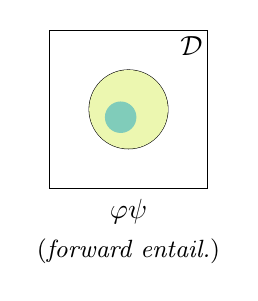
\begin{tikzpicture}
    \def\vennA{(-0.1,-0.1) circle (0.2)}
    \def\vennB{(-0.0,-0.0) circle (0.5)}

    \draw \vennB node [below] {};
    \draw \vennA node [above] {};
    \begin{scope}
      \fill[fill=light] \vennB;
    \end{scope}
    \begin{scope}
      \fill[fill=dark] \vennA;
    \end{scope}
    
    \frameVenn
    \draw (0, -1.3) node {$\varphi \forward \psi$};
    \relName{forward entail.}
  \end{tikzpicture}
}

\newcommand\reverseVenn{
  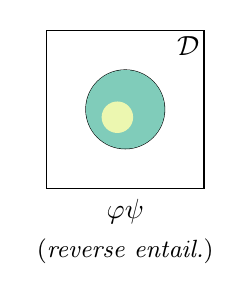
\begin{tikzpicture}
    \def\vennA{(-0.1,-0.1) circle (0.2)}
    \def\vennB{(0.0,0.0) circle (0.5)}
    
    \draw \vennB node [below] {};
    \draw \vennA node [above] {};
    \begin{scope}
      \fill[fill=dark] \vennB;
    \end{scope}
    \begin{scope}
      \fill[fill=light] \vennA;
    \end{scope}
    
    \frameVenn
    \draw (0, -1.3) node {$\varphi \reverse \psi$};
    \relName{reverse entail.}
  \end{tikzpicture}
}

\newcommand\negateVenn{
  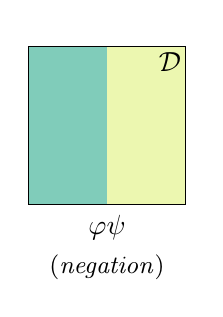
\begin{tikzpicture}
    \def\vennA{(0,-1) rectangle (1,1)}
    \def\vennB{(-1,-1) rectangle (0,1)}
    
    \draw \vennB node [below] {};
    \draw \vennA node [above] {};
    \begin{scope}
      \fill[fill=dark] \vennB;
    \end{scope}
    \begin{scope}
      \fill[fill=light] \vennA;
    \end{scope}
    
    \frameVenn
    \draw (0, -1.3) node {$\varphi \negate \psi$};
    \relName{negation}
  \end{tikzpicture}
}

\newcommand\alternateVenn{
  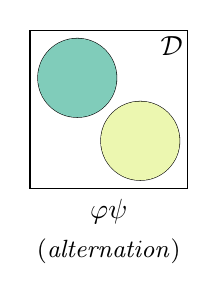
\begin{tikzpicture}
    \def\vennA{(0.4,-0.4) circle (0.5)}
    \def\vennB{(-0.4,0.4) circle (0.5)}
    
    \draw \vennB node [below] {};
    \draw \vennA node [above] {};
    \begin{scope}
      \fill[fill=dark] \vennB;
    \end{scope}
    \begin{scope}
      \fill[fill=light] \vennA;
    \end{scope}
    
    \frameVenn
    \draw (0, -1.3) node {$\varphi \alternate \psi$};
    \relName{alternation}
  \end{tikzpicture}
}

\newcommand\coverVenn{
  \begin{tikzpicture}
    \def\vennA{(-0.2,-1) rectangle (1,1)}
    \def\vennB{(-1,-1) rectangle (0.2,1)}
    
    \draw \vennB node [below] {};
    \draw \vennA node [above] {};
    \begin{scope}
      \fill[fill=dark] \vennB;
    \end{scope}
    \begin{scope}
      \fill[fill=light] \vennA;
    \end{scope}
    \begin{scope}
      \clip \vennA;
      \fill[pattern=north west lines, pattern color=dark] \vennB;
    \end{scope}
    
    \frameVenn
    \draw (0, -1.3) node {$\varphi \cover \psi$};
    \relName{cover}
  \end{tikzpicture}
}

\newcommand\independentVenn{
  \begin{tikzpicture}
    \def\vennA{(0.25,-0.25) circle (0.5)}
    \def\vennB{(-0.25,0.25) circle (0.5)}
    
    \draw \vennB node [below] {};
    \draw \vennA node [above] {};
    \begin{scope}
      \fill[fill=dark] \vennB;
    \end{scope}
    \begin{scope}
      \fill[fill=light] \vennA;
    \end{scope}
    \begin{scope}
      \clip \vennA;
      \fill[pattern=north west lines, pattern color=dark] \vennB;
    \end{scope}
    
    \frameVenn
    \draw (0, -1.3) node {$\varphi \independent \psi$};
    \relName{independence}
  \end{tikzpicture}
}



%
% -----
% NatLog Monotonicity
% -----
%
\def\monoHeader{
  \begin{tikzpicture}[node distance=0cm,
                      start chain=going below,
                      punktchain/.style={
                        rectangle, 
                        rounded corners, 
                        draw=black, very thick,
                        text width=6em, 
                        minimum height=2em, 
                        text centered, 
                        on chain},
                      black/.style={
                        text width=6em, 
                        minimum height=3.25ex, 
                        text centered, 
                        text=black,
                        on chain},
                      gray/.style={
                        text width=6em, 
                        minimum height=3.25ex, 
                        text centered, 
                        text=gray,
                        on chain},
                      ]
}
\newcommand\monoUp[4]{
  \monoHeader
    \node[black]{#4};
    \node[black]{#3};
    \node[punktchain, color=blue]{$\uparrow$ #2};
    \node[gray]{#1};
  \end{tikzpicture}
}

\newcommand\monoDown[4]{
  \monoHeader
    \node[gray]{#4};
    \node[gray]{#3};
    \node[punktchain, color=blue]{$\downarrow$ #2};
    \node[black]{#1};
  \end{tikzpicture}
}

\newcommand\monoUpR[4]{
  \monoHeader
    \node[gray]{#4};
    \node[gray]{#3};
    \node[punktchain, color=blue]{$\uparrow$ #2};
    \node[black]{#1};
  \end{tikzpicture}
}

\newcommand\monoDownR[4]{
  \monoHeader
    \node[black]{#4};
    \node[black]{#3};
    \node[punktchain, color=blue]{$\downarrow$ #2};
    \node[gray]{#1};
  \end{tikzpicture}
}

\newcommand\monoFlat[4]{
  \monoHeader
    \node[gray]{#4};
    \node[gray]{#3};
    \node[punktchain, color=blue]{$---$ #2};
    \node[gray]{#1};
  \end{tikzpicture}
}

\def\monoHeaderPoster{
  \begin{tikzpicture}[node distance=0cm,
                      start chain=going below,
                      punktchain/.style={
                        rectangle, 
                        rounded corners, 
                        draw=black, very thick,
                        text width=3em, 
                        minimum height=2em, 
                        text centered, 
                        on chain},
                      black/.style={
                        text width=3em, 
                        minimum height=3.25ex, 
                        text centered, 
                        text=black,
                        on chain},
                      gray/.style={
                        text width=3em, 
                        minimum height=3.25ex, 
                        text centered, 
                        text=gray,
                        on chain},
                      ]
}
\newcommand\monoUpPoster[4]{
  \monoHeaderPoster
    \node[black]{#4};
    \node[black]{#3};
    \node[punktchain, color=blue]{$\uparrow$ #2};
    \node[gray]{#1};
  \end{tikzpicture}
}

\newcommand\monoDownPoster[4]{
  \monoHeaderPoster
    \node[gray]{#4};
    \node[gray]{#3};
    \node[punktchain, color=blue]{$\downarrow$ #2};
    \node[black]{#1};
  \end{tikzpicture}
}

\newcommand\monoFlatPoster[4]{
  \monoHeaderPoster
    \node[gray]{#4};
    \node[gray]{#3};
    \node[punktchain, color=blue]{$---$ #2};
    \node[gray]{#1};
  \end{tikzpicture}
}

%
% -----
% Graph Fragments
% -----
%

\newcommand\exampleTreeImpl[5]{
  \setstyles
  \tikzstyle{level 2}=[level distance=1.5cm, sibling distance=3.5cm]
  \begin{tikzpicture}[grow=down, sloped]
    \node[fact] {\w{\gray{#1}}}
    child {
      node[boxfact] {\w{#2?}}
        child {
          node[#5] {\w{#3}} 
          edge from parent [strongPath] node[above] {}
        }
        child {
          node[fact] {\w{#4}} 
        }
        child {
          node[fact] {$\dots$}
        }
    };
  \end{tikzpicture}
}
\newcommand\exampleTree[4]{\exampleTreeImpl{#1}{#2}{#3}{#4}{fact}}
\newcommand\exampleTreeEnd[4]{\exampleTreeImpl{#1}{#2}{#3}{#4}{sink}}

\def\exampleStepOne{\exampleTree{ROOT \\ $~$}
                                {No carnivores eat animals}
                                {\darkblue{The} carnivores eat animals}
                                {No \darkblue{animals} eat animals}}
\def\exampleStepTwo{\exampleTree{No carnivores eat animals}
                                {The carnivores eat animals}
                                {The \darkblue{feline} eats animals}
                                {\darkblue{All} carnivores eat animals}}
\def\exampleStepThree{\exampleTree{The carnivores eat animals}
                                  {The feline eats animals}
                                  {The \darkblue{cat} eats animals}
                                  {The cat eats \darkblue{chordate}}}
\def\exampleStepFour{\exampleTree{The feline eats animals}
                                 {The cat eats animals}
                                 {The cat eats \darkblue{chordates}}
                                 {The \darkblue{kitty} eats animals}}
\def\exampleStepFive{\exampleTree{The cat eats animals}
                                 {The cat eats chordates}
                                 {The cat eats \darkblue{mice}}
                                 {The cat eats \darkblue{dogs}}}
\def\exampleStepSix{\exampleTreeEnd{The cat eats chordates}
                                   {The cat eats mice}
                                   {The cat ate \darkblue{a} mouse}
                                   {The \darkblue{kitty} eats mice}}
\def\exampleStepEnd{
  \setstyles
  \begin{tikzpicture}[grow=down, sloped]
  \node[sink](main) {\w{The cat ate a mouse}};
  \end{tikzpicture}
}

\def\exampleInsertions{\exampleTree{The cat eats chordates}
                                   {The cat ate mouse?}
                                   {The cat ate \textbf{a} mouse}
                                   {The cat ate \textbf{catnip} mice}}

%
% -----
% Fact Trie
% -----
%
\def\settriestyles{
  \tikzstyle{level 1}=[level distance=2.5cm, sibling distance=2.0cm]
  \tikzstyle{level 2}=[level distance=2.5cm, sibling distance=2.0cm]
  \tikzstyle{level 3}=[level distance=2.5cm, sibling distance=2.0cm]
  \tikzstyle{level 4}=[level distance=2.5cm, sibling distance=2.0cm]
  \tikzstyle{trie} = [text width=1em, text centered]
  \tikzstyle{sink} = [text width=7em, text centered, 
                      rectangle, draw=blue]
  \tikzstyle{othersink} = [text width=5em, text centered, 
                      rectangle, draw=blue]
  \tikzset{
    goodPath/.style={draw=blue}
  }
  \tikzset{
    path/.style={draw=black, line width=1pt}
  }
  \tikzset{
    strongPath/.style={draw=blue, line width=3pt}
  }
  \tikzset{
    dotpath/.style={draw=black, line width=1pt, dashed}
  }
}

\newcommand\factTrie[3]{
\begin{tikzpicture}[grow=right, sloped]
  \settriestyles
  \def\dot{\Huge{\ensuremath{\cdot}}}

  \node[trie] {\dot}
    child {
      node[trie] {\dot} 
      edge from parent [path] node[above] {\w{Socrates}}
    }
    child {
      node[trie] {\dot} 
      child {
        node[trie] {\dot} 
        edge from parent [path] node[above] {\w{fish}}
      }
      child {
        node[trie] {\dot} 
        child {
          node[trie] {\dot} 
          edge from parent [path] node[above] {\w{sleeps}}
        }
        child {
          node[trie] {\dot} 
          edge from parent [path] node[above] {\w{likes}}
        }
        child {
          node[trie] {\dot}
            child {
              node[trie] {\dot} 
              edge from parent [#3] node[above] {\w{a}}
            }
            child {
              node[trie] {\dot} 
              edge from parent [#2] node[above] {\w{my}}
            }
            child {
              node[trie] {\dot}
              edge from parent [#1] node[above] {\w{catnip}}
            }
          edge from parent [strongPath] node[above] {\w{ate}}
        }
        edge from parent [strongPath] node[above] {\w{cat}}
      }
      child {
        node[trie] {\dot}
        edge from parent [path] node[above] {\w{economist}}
      }
      edge from parent [strongPath] node[above] {\w{The}};
    }
    child {
      node[trie] {\dot}
      edge from parent [path] node[above] {\w{All}}
    };

\end{tikzpicture}
}


%
% -----
% Lattice
% -----
%
\newcommand\lattice{
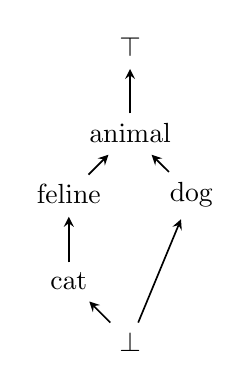
\begin{tikzpicture}[->,>=stealth,shorten >=1pt,auto,node distance=1.1cm,
                    semithick]
  \node[] (top)                            {$\top$};
  \node[] (animal) [below of=top]          {\w{animal}};
  \node[] (feline) [below left of=animal]  {\w{feline}};
  \node[] (cat)    [below of=feline]       {\w{cat}};
  \node[] (dog)    [below right of=animal] {\w{dog}};
  \node[] (bot)    [below right of=cat]    {$\bot$};

  \path (animal) edge (top)
        (feline) edge (animal)
        (cat)    edge (feline)
        (dog)    edge (animal)
        (bot)    edge (cat)
                 edge (dog);

\end{tikzpicture}
}



%
% Standalone figures
%
\newcommand\polarityOne{
  \monoHeader
    \node[black]{animal};
    \node[black]{feline};
    \node[punktchain,color=blue]{cat};
    \node[black]{house cat};
  \end{tikzpicture}
}
\newcommand\polarityTwo{
  \monoUp{house cat}{cat}{feline}{animal}
}
\newcommand\polarityThree{
  \monoUp{cat}{feline}{animal}{living thing}
}
\newcommand\polarityFour{
  \monoUp{feline}{animal}{living thing}{thing}
}
\newcommand\polarityFive{
  \monoDown{feline}{animal}{living thing}{thing}
}
\newcommand\polaritySix{
  \monoDown{house cat}{cat}{feline}{animal}
}

\newcommand\conceptnetResults{
  \begin{tabular}{lcc}
    System             & P     & R    \\
    \hline
    Direct Lookup      & 100.0 & \textbf{12.1} \\
    NaturalLI Only     & 88.8  & 40.1 \\
    NaturalLI          & 90.6  & \textbf{49.1} \\
  \end{tabular}
}


%
% Dependency Trees
%
\def\treeBlank{
  \begin{dependency}[text only label, label style={above}]
    \begin{deptext}[column sep=-0.00cm]
      Born \& in \& a \& small \& town \&[-1ex] , \& she \& took \& the \&
        midnight \& train \& going \& anywhere \&[-1ex] . \\
    \end{deptext}
    \depedge[edge unit distance=1.75ex]{1}{5}{nmod:in}
    \depedge[edge unit distance=1.5ex]{5}{4}{amod}
    \depedge[edge unit distance=2.25ex]{5}{3}{det}
    \depedge[edge unit distance=1.4ex]{8}{1}{advcl}
    \depedge[edge unit distance=2.25ex]{8}{7}{nsubj}
    \depedge[edge unit distance=2.25ex]{8}{11}{dobj}
    \depedge[edge unit distance=1.5ex]{11}{10}{nn}
    \depedge[edge unit distance=1.9ex]{11}{9}{det}
    \depedge[edge unit distance=1.5ex]{11}{12}{advcl}
    \depedge[edge unit distance=1.5ex]{12}{13}{dobj}
  \end{dependency}
}

\def\treeEdge{
  \begin{dependency}[text only label, label style={above}]
    \begin{deptext}[column sep=-0.00cm]
      Born \& in \& a \& small \& town \&[-1ex] , \& she \& took \& the \&
        midnight \& train \& going \& anywhere \&[-1ex] . \\
    \end{deptext}
    \depedge[edge unit distance=1.75ex]{1}{5}{nmod:in}
    \depedge[edge unit distance=1.5ex]{5}{4}{amod}
    \depedge[edge unit distance=2.25ex]{5}{3}{det}
    \depedge[edge unit distance=1.4ex, edge style={darkred!60!black,thick,densely dotted}]{8}{1}{\textbf{\darkred{advcl}}}
    \depedge[edge unit distance=2.25ex]{8}{7}{nsubj}
    \depedge[edge unit distance=2.25ex]{8}{11}{dobj}
    \depedge[edge unit distance=1.5ex]{11}{10}{nn}
    \depedge[edge unit distance=1.9ex]{11}{9}{det}
    \depedge[edge unit distance=1.5ex]{11}{12}{advcl}
    \depedge[edge unit distance=1.5ex]{12}{13}{dobj}
  \end{dependency}
}

\def\treeSubj{
  \begin{dependency}[text only label, label style={above}]
    \begin{deptext}[column sep=-0.00cm]
      Born \& in \& a \& small \& town \&[-1ex] , \& \darkred{she} \& took \& the \&
        midnight \& train \& going \& anywhere \&[-1ex] . \\
    \end{deptext}
    \depedge[edge unit distance=1.75ex]{1}{5}{nmod:in}
    \depedge[edge unit distance=1.5ex]{5}{4}{amod}
    \depedge[edge unit distance=2.25ex]{5}{3}{det}
    \depedge[edge unit distance=1.4ex, edge style={darkred!60!black,thick,densely dotted}]{8}{1}{\textbf{\darkred{advcl}}}
    \depedge[edge unit distance=2.25ex, edge style={blue!60!black,thick}]{8}{7}{\darkblue{nsubj}}
    \depedge[edge unit distance=2.25ex]{8}{11}{dobj}
    \depedge[edge unit distance=1.5ex]{11}{10}{nn}
    \depedge[edge unit distance=1.9ex]{11}{9}{det}
    \depedge[edge unit distance=1.5ex]{11}{12}{advcl}
    \depedge[edge unit distance=1.5ex]{12}{13}{dobj}
  \end{dependency}
}

\def\treeObj{
  \begin{dependency}[text only label, label style={above}]
    \begin{deptext}[column sep=-0.00cm]
      Born \& in \& a \& small \& town \&[-1ex] , \& she \& took \& \darkred{the} \&
        \darkred{midnight} \& \darkred{train} \& \darkred{going} \& 
        \darkred{anywhere} \&[-1ex] . \\
    \end{deptext}
    \depedge[edge unit distance=1.75ex]{1}{5}{nmod:in}
    \depedge[edge unit distance=1.5ex]{5}{4}{amod}
    \depedge[edge unit distance=2.25ex]{5}{3}{det}
    \depedge[edge unit distance=1.4ex, edge style={darkred!60!black,thick,densely dotted}]{8}{1}{\textbf{\darkred{advcl}}}
    \depedge[edge unit distance=2.25ex]{8}{7}{nsubj}
    \depedge[edge unit distance=2.25ex, edge style={blue!60!black,thick}]{8}{11}{\darkblue{dobj}}
    \depedge[edge unit distance=1.5ex]{11}{10}{nn}
    \depedge[edge unit distance=1.9ex]{11}{9}{det}
    \depedge[edge unit distance=1.5ex]{11}{12}{advcl}
    \depedge[edge unit distance=1.5ex]{12}{13}{dobj}
  \end{dependency}
}

\def\treeParent{
  \begin{dependency}[text only label, label style={above}]
    \begin{deptext}[column sep=-0.00cm]
      Born \& in \& a \& small \& town \&[-1ex] , \& she \& \darkred{took} \& the \&
        midnight \& train \& going \& anywhere \&[-1ex] . \\
    \end{deptext}
    \depedge[edge unit distance=1.75ex]{1}{5}{nmod:in}
    \depedge[edge unit distance=1.5ex]{5}{4}{amod}
    \depedge[edge unit distance=2.25ex]{5}{3}{det}
    \depedge[edge unit distance=1.4ex, edge style={darkred!60!black,thick,densely dotted}]{8}{1}{\textbf{\darkred{advcl}}}
    \depedge[edge unit distance=2.25ex]{8}{7}{nsubj}
    \depedge[edge unit distance=2.25ex]{8}{11}{dobj}
    \depedge[edge unit distance=1.5ex]{11}{10}{nn}
    \depedge[edge unit distance=1.9ex]{11}{9}{det}
    \depedge[edge unit distance=1.5ex]{11}{12}{advcl}
    \depedge[edge unit distance=1.5ex]{12}{13}{dobj}
  \end{dependency}
}

\def\treeYield{
  \begin{dependency}[text only label, label style={above}]
    \begin{deptext}[column sep=-0.00cm]
      Dentists \& suggest \& that \& \darkgreen{you} \& \darkgreen{should} \& 
      \darkgreen{brush} \& \darkgreen{your} \& \darkgreen{teeth} \&[-1ex] . \\
    \end{deptext}
    \depedge[edge unit distance=2.5ex, edge style={darkred!60!black,thick,densely dotted}]{2}{6}{\textbf{\darkred{ccomp}}}
    \depedge[edge unit distance=1.75ex]{2}{1}{nsubj}
    \depedge[edge unit distance=2.25ex]{6}{3}{mark}
    \depedge[edge unit distance=2.25ex]{6}{4}{nsubj}
    \depedge[edge unit distance=2.25ex]{6}{5}{aux}
    \depedge[edge unit distance=2.25ex]{6}{8}{dobj}
    \depedge[edge unit distance=1.5ex]{8}{7}{nmod:poss}
  \end{dependency}
}

\def\treeYieldSubj{
  \begin{dependency}[text only label, label style={above}]
    \begin{deptext}[column sep=-0.00cm]
      \darkgreen{Born} \& \darkgreen{in} \& \darkgreen{Hawaii} \& , \& \darkgreen{Obama} \& 
      is \& a \& US \& citizen \&[-1ex] .\\
    \end{deptext}
    \depedge[edge unit distance=1.50ex, edge style={darkred!60!black,thick,densely dotted}]{9}{1}{\textbf{\darkred{advcl}}}
    \depedge[edge unit distance=2.25ex, edge style={blue!60!black,thick}]{9}{5}{\darkblue{nsubj}}
    \depedge[edge unit distance=2.25ex]{9}{6}{cop}
    \depedge[edge unit distance=2.25ex]{9}{7}{det}
    \depedge[edge unit distance=2.25ex]{9}{8}{amod}
    \depedge[edge unit distance=2.25ex]{1}{3}{nmod:in}
  \end{dependency}
}

\def\treeYieldObj{
  \begin{dependency}[text only label, label style={above}]
    \begin{deptext}[column sep=-0.00cm]
      I \& persuaded \& \darkgreen{Fred} \& to \& \darkgreen{leave} \& 
      \darkgreen{the} \& \darkgreen{room} \&[-1ex] .\\
    \end{deptext}
    \depedge[edge unit distance=2.00ex, edge style={darkred!60!black,thick,densely dotted}]{2}{5}{\textbf{\darkred{xcomp}}}
    \depedge[edge unit distance=2.25ex, edge style={blue!60!black,thick}]{2}{3}{\darkblue{dobj}}
    \depedge[edge unit distance=2.25ex]{2}{1}{nsubj}
    \depedge[edge unit distance=2.25ex]{5}{4}{mark}
    \depedge[edge unit distance=2.50ex]{5}{7}{dobj}
    \depedge[edge unit distance=2.25ex]{7}{6}{det}
  \end{dependency}
}

\def\treeYieldRoot{
  \begin{dependency}[text only label, label style={above}]
    \begin{deptext}[column sep=-0.00cm]
      \darkgreen{Obama} \&[-1ex] , \& \darkgreen{our} \& \darkgreen{44th} \& 
      \darkgreen{president} \&[-1ex] . \\
    \end{deptext}
    \depedge[edge unit distance=2.00ex, edge style={darkred!60!black,thick,densely dotted}]{1}{5}{\textbf{\darkred{appos}}}
    \depedge[edge unit distance=2.25ex]{4}{2}{nmod:poss}
    \depedge[edge unit distance=2.25ex]{4}{3}{amod}
  \end{dependency}
}

\newcommand\openieKBPBase{
  \def\bell{\raisebox{-2.5mm}{
\includegraphics[height=5mm]{../img/bell.png}}}
  \def\whistle{\raisebox{-2.5mm}{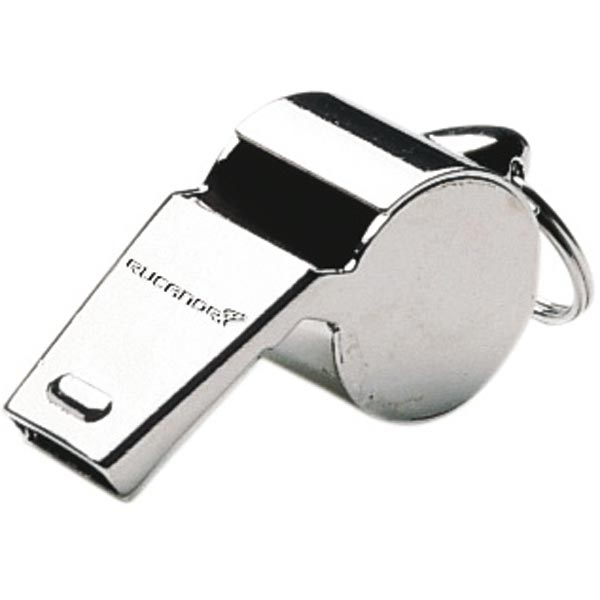
\includegraphics[height=5mm]{../img/whistle.jpg}}}
  \begin{tabular}{lrrr}
  \hline
  \textbf{System}                & \multicolumn{1}{c}{\textbf{P}}    
                                 & \multicolumn{1}{c}{\textbf{R}}    
                                 & \multicolumn{1}{c}{\textbf{F$_1$}} \\
  \hline
  UW Submission                   & 69.8          & 11.4          & 19.6 \\
  Ollie                           & 57.7          & 11.8          & 19.6 \\
  \darkblue{Our System}           & \darkblue{61.9} & \darkblue{13.9} & \darkblue{22.7} \\
  \hline
  \end{tabular}
}

\newcommand\openieKBPFull{
  \def\bell{\raisebox{-2.5mm}{
\includegraphics[height=5mm]{../img/bell.png}}}
  \def\whistle{\raisebox{-2.5mm}{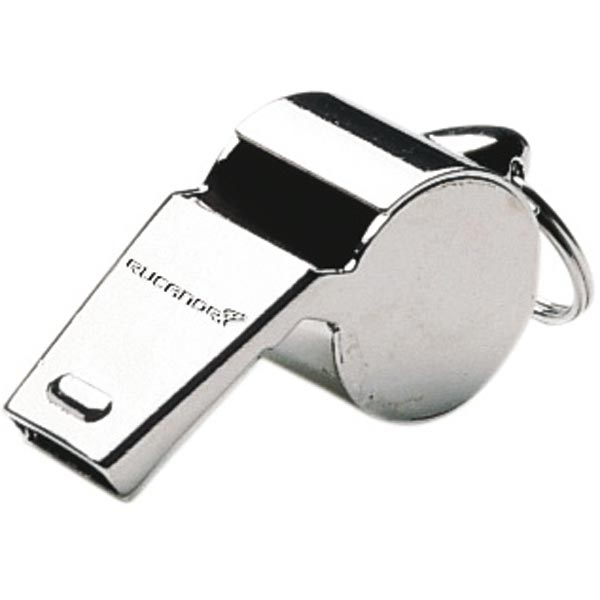
\includegraphics[height=5mm]{../img/whistle.jpg}}}
  \begin{tabular}{lrrr}
  \hline
  \textbf{System}                & \multicolumn{1}{c}{\textbf{P}}    
                                 & \multicolumn{1}{c}{\textbf{R}}    
                                 & \multicolumn{1}{c}{\textbf{F$_1$}} \\
  \hline
  UW Submission                   & 69.8          & 11.4          & 19.6 \\
  Ollie                           & 57.7          & 11.8          & 19.6 \\
  \darkblue{Our System}           & \darkblue{61.9} & \darkblue{13.9} & \darkblue{22.7} \\
  \hline
  Median Team                     &               &               & 18.6 \\
  \darkblue{Our System} + \bell\ + \whistle  & \darkblue{58.6} & \darkblue{18.6} & \darkblue{28.3} \\
  Top Team                        & 45.7          & 35.8          & 40.2 \\
  \hline
  \end{tabular}
}
